\documentclass[fleqn,onecolumn,a4paper,12pt,titlepage]{article}
\usepackage[showcrop]{geometry}
\geometry{textheight=25.0cm,textwidth=17.0cm,headheight=3cm,headsep=0.5em}%hmargin=4.2cm
\usepackage{graphicx}%[dvips,pdftex]
\usepackage{amssymb}
\usepackage{amsmath}%centertags
\usepackage[T1]{fontenc}
\usepackage[polish]{babel}
\usepackage{float}
\usepackage[final]{listingsutf8}
\usepackage{fancyhdr}
\usepackage{tikz}
\usepackage{caption}
\usepackage{datetime2}
\usepackage{enumitem}
\usepackage{blindtext}
\usepackage{hyperref}

\pagestyle{fancy}
\fancyfoot[L,R]{\tiny{\texttt{\symbol{64}}  built: \today{} at \DTMcurrenttime}} 

% --- definicja stylu C++ ---
\definecolor{codebg}{RGB}{245,245,244}
\definecolor{comment}{RGB}{0,128,0}
\definecolor{keyword}{RGB}{0,0,180}
\definecolor{string}{RGB}{163,21,21}
\definecolor{linenumber}{RGB}{120,120,120}

\lstdefinestyle{cppstyle}{
    language=C++,
    backgroundcolor=\color{codebg},
    basicstyle=\ttfamily\small,
    keywordstyle=\color{keyword}\bfseries,
    commentstyle=\color{comment}\itshape,
    stringstyle=\color{string},
    numberstyle=\tiny\color{linenumber},
    numbers=left,
    stepnumber=1,
    numbersep=10pt,
    tabsize=4,
    showspaces=false,
    showstringspaces=false,
    breaklines=true,
    breakatwhitespace=true,
    frame=single,
    rulecolor=\color{black},
    captionpos=b
}

\lstset{style=cppstyle}

\begin{document}

\begin{titlepage}
    
\includegraphics[width=0.25\textwidth]{logo_kia.png}\par\vspace{3cm}
    \centering
    {\LARGE \textsc{Zaawansowane Programowanie w Języku C++} \par}
    \vspace{2cm}
    {\Large \textsc{Raport z wykonania projektu} \par} % NALEŻY UZUPEŁNIĆ
    \vspace{2cm}
    {\textsc{Plane Manager} \par} % NALEŻY UZUPEŁNIĆ
    \vfill
    Hubert Lech $-$ 177827 $-$ L09 \par % NALEŻY UZUPEŁNIĆ
    \vspace{2cm}
    {\large {\today} \par}
\end{titlepage}

\section*{Wstęp}

Plane Manager to desktopowa aplikacja do zarządzania niewielką flotą lotniczą, zaprojektowana tak, aby w prosty i czytelny sposób zarządzać informacjami o samolotach oraz ich wykorzystaniu w zaplanowanych lotach. Z perspektywy użytkownika aplikacja działa jak mały panel administracyjny: można dodać samolot, uzupełnić jego parametry techniczne (np. długość, liczba silników, pojemność pasażerska, prędkość i pułap), zmienić status (np. dostępny lub w serwisie), a następnie zaplanować lot pomiędzy wybranymi lotniskami. Podczas rezerwacji i edycji lotów aplikacja pilnuje porządku w terminarzu --- sprawdza, czy daty są poprawne oraz czy nie dochodzi do nakładania się rezerwacji dla tego samego samolotu; dodatkowo uwzględnia sytuację, w której samolot jest wyłączony z użytku (np. znajduje się w serwisie). Poza samym planowaniem lotów dostępny jest też widok podsumowań: statystyki floty (ile maszyn jest dostępnych, w locie lub w serwisie), a także informacje takie jak najdłuższy i najkrótszy samolot czy największa i najmniejsza liczba pasażerów. Dzięki temu jednym spojrzeniem można ocenić, w jakiej kondycji jest flota i jakie maszyny wyróżniają się parametrami.
Projekt został zrealizowany w oparciu o framework Qt. Logika aplikacji i komunikacja z bazą danych zostały napisane w C++, natomiast interfejs użytkownika przygotowano w QML, co pozwoliło uzyskać responsywny i miły dla oka układ widoków. Dane przechowywane są w relacyjnej bazie PostgreSQL uruchomionej w środowisku Supabase, a dostęp do nich realizowany jest przez moduł QtSql.


\newpage

\section*{Baza danych}

Po uruchomieniu aplikacji nawiązywane jest połączenie z bazą danych PostgreSQL działającą w Supabase. Za ten etap odpowiada klasa \texttt{DatabaseManager}, która konfiguruje połączenie w QtSql z użyciem sterownika \texttt{QPSQL}. Parametry dostępu nie są wpisane na stałe w kodzie --- aplikacja pobiera je ze zmiennych środowiskowych (m.in. \texttt{DB\_HOST}, \texttt{DB\_NAME}, \texttt{DB\_USER}, \texttt{DB\_PASS}, \texttt{DB\_PORT}), co ułatwia przenoszenie projektu pomiędzy komputerami i ogranicza ryzyko przypadkowego ujawnienia danych dostępowych w repozytorium. Dodatkowo ustawione zostały opcje połączenia takie jak \texttt{keepalives} i limit czasu na nawiązanie połączenia, aby zmniejszyć prawdopodobieństwo rozłączania sesji na warstwie poolera.

Warstwa danych aplikacji została oparta o relacyjną bazę PostgreSQL uruchomioną w środowisku Supabase. Taki wybór pozwala przechowywać dane w sposób uporządkowany (tabele i relacje), a jednocześnie ułatwia dalszą rozbudowę projektu o kolejne encje. Po stronie aplikacji połączenie realizowane jest przez QtSql z wykorzystaniem sterownika QPSQL, a zapytania wykonywane są w większości jako \texttt{prepared statements} (\texttt{QSqlQuery::prepare} oraz \texttt{bindValue}), co poprawia czytelność kodu i ogranicza ryzyko błędów związanych z wklejaniem wartości do SQL.

W projekcie baza danych składa się z trzech głównych tabel, które odzwierciedlają podstawowe elementy domeny:
\begin{itemize}[leftmargin=*]
    \item \textbf{planes} --- przechowuje informacje o samolotach (marka, model, status oraz parametry techniczne takie jak długość, liczba silników, pojemność, prędkość maksymalna i pułap). Rekordy identyfikowane są kluczem głównym \texttt{id}.
    \item \textbf{airports} --- zawiera lotniska wraz z kodem ICAO, nazwą oraz współrzędnymi geograficznymi (szerokość i długość). Rekordy identyfikowane są kluczem \texttt{id}; kod \texttt{icao\_code} jest wykorzystywany do czytelnej prezentacji w UI.
    \item \textbf{flights} --- reprezentuje zaplanowane loty: wskazuje samolot (\texttt{plane\_id}) oraz lotniska wylotu i przylotu (\texttt{departure\_airport\_id}, \texttt{arrival\_airport\_id}), a także przedział czasowy lotu (\texttt{start\_time}, \texttt{end\_time}).
\end{itemize}

Relacje pomiędzy tabelami są naturalne dla problemu: jeden samolot może wystąpić w wielu lotach (relacja 1--N), a każdy lot wskazuje dwa lotniska (wylotu i przylotu). Schemat relacji przedstawiono na diagramie~\ref{fig:db_erd}. W czasie implementacji ważne było również poprawne przetwarzanie czasu --- wartości czasowe zapisywane są w bazie w UTC (aplikacja dokonuje konwersji na UTC przy zapisie oraz na czas lokalny przy prezentacji), a przy dodawaniu/edycji lotu wykonywana jest walidacja terminów, w tym wykrywanie nakładania się rezerwacji dla tego samego samolotu.

\begin{figure}[H]%
    \centering
    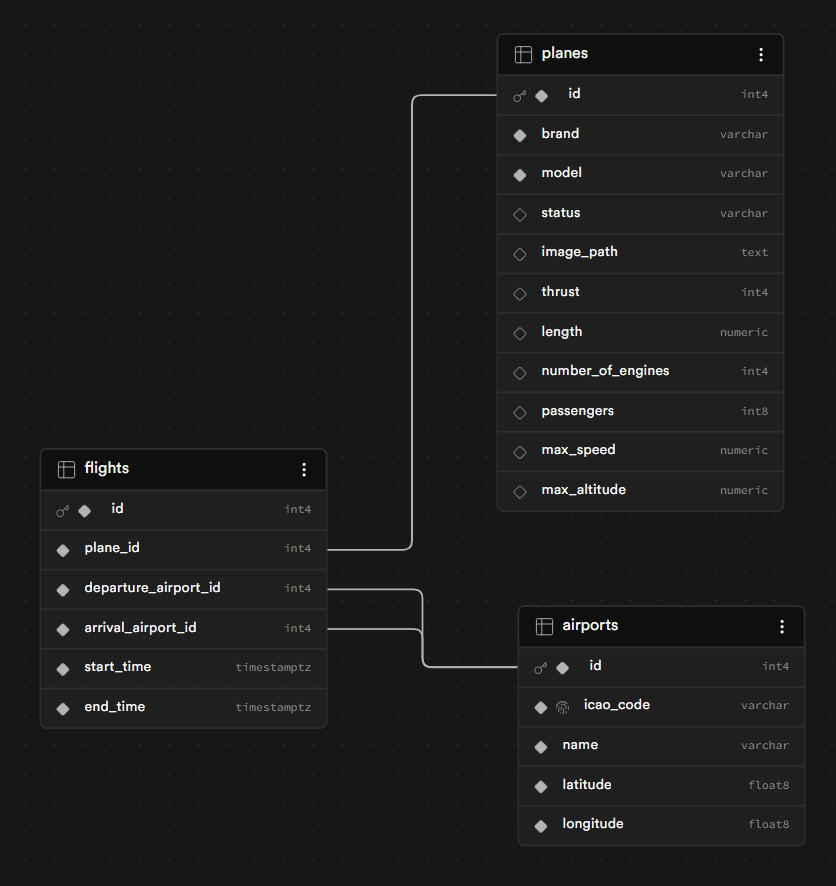
\includegraphics[width=0.9\textwidth]{baza.png}
    \caption{Diagram relacji bazy danych (ERD)}
    \label{fig:db_erd}
\end{figure}

Poniżej przedstawiono przykładowe fragmenty kodu odpowiedzialne za operacje CRUD (Create, Read, Update, Delete) na głównych encjach aplikacji: samolotach, lotniskach oraz lotach.

\textbf{Samoloty (planes).} Listing~\ref{lst:crud_planes} pokazuje kompletny zestaw operacji na tabeli \texttt{planes}. Dodawanie i aktualizacja realizowane są poprzez zapytania parametryzowane (\texttt{prepare} + \texttt{bindValue}), co upraszcza przekazywanie wielu pól technicznych samolotu i zachowuje porządek w kodzie. Odczyt (\texttt{getAllPlanes}) pobiera listę samolotów w postaci \texttt{QVariantList} z mapami, gotową do bezpośredniego użycia w warstwie QML. Dodatkowo w zapytaniu odczytu zastosowano logikę w SQL (\texttt{CASE} + \texttt{EXISTS}), aby status samolotu w UI uwzględniał to, czy maszyna aktualnie bierze udział w locie.

\lstinputlisting[
    caption={Operacje CRUD dla samolotów (tabela \texttt{planes})},
    label={lst:crud_planes},
    inputencoding=cp1250,
    firstline=14,
    lastline=115
]{../src/PlaneManager.cpp}

\textbf{Lotniska (airports).} Listing~\ref{lst:crud_airports} prezentuje podstawowe operacje CRUD dla lotnisk. Model danych jest tu prosty (kod ICAO, nazwa oraz współrzędne), dlatego zapytania są krótkie i czytelne: dodanie rekordu, pobranie listy posortowanej po kodzie ICAO, edycja oraz usunięcie po identyfikatorze \texttt{id}. Tak przygotowana warstwa pozwala UI szybko zasilać listy wyboru lotnisk oraz przechowywać dane potrzebne np. do prezentacji na mapie.

\lstinputlisting[
    caption={Operacje CRUD dla lotnisk (tabela \texttt{airports})},
    label={lst:crud_airports},
    inputencoding=cp1250,
    firstline=13,
    lastline=74
]{../src/AirportManager.cpp}

\textbf{Loty (flights).} Listing~\ref{lst:crud_flights} zawiera operacje CRUD dla lotów, ale w tym przypadku sama „goła” manipulacja danymi nie wystarcza --- najważniejsza jest walidacja reguł biznesowych. Przed dodaniem lub aktualizacją lotu aplikacja sprawdza m.in. czy wybrany samolot nie ma statusu serwisowego oraz czy jego terminarz nie koliduje z innymi lotami (nakładanie się przedziałów czasu). Odczyt listy lotów korzysta z \texttt{JOIN}, aby poza identyfikatorami zwrócić też czytelne dane (np. marka/model samolotu, kody ICAO i współrzędne lotnisk), a dodatkowo wylicza status lotu (zaplanowany/w trakcie/zakończony) na podstawie czasu.

\lstinputlisting[
    caption={Operacje CRUD dla lotów (tabela \texttt{flights}) wraz z walidacją terminów},
    label={lst:crud_flights},
    inputencoding=cp1250,
    firstline=1,
    lastline=226
]{../src/FlightManager.cpp}


\newpage

\section*{Struktura aplikacji}

Aplikacja została zbudowana w typowym dla Qt podziale na warstwę logiki w C++ oraz warstwę interfejsu w QML. W praktyce oznacza to, że widoki (lista samolotów, lista lotów, statystyki itd.) są zdefiniowane w QML, natomiast pobieranie i modyfikacja danych odbywa się w C++ przez QtSql. Ważnym elementem architektury jest sposób komunikacji C++--QML: w tym projekcie „klasy” nie pełnią roli tradycyjnych obiektów domenowych (z bogatym modelem typów i osobnymi klasami \texttt{Plane}/\texttt{Flight}/\texttt{Airport}), tylko są lekkimi \textbf{serwisami} (menedżerami) udostępniającymi zestaw metod do UI.

\subsection*{Warstwa C++: serwisy (menedżery)}

W części C++ znajdują się klasy dziedziczące po \texttt{QObject}, których głównym zadaniem jest udostępnienie API do QML oraz komunikacja z bazą danych:
\begin{itemize}[leftmargin=*]
    \item \textbf{\texttt{DatabaseManager}} --- inicjalizuje połączenie z PostgreSQL (Supabase) przez sterownik \texttt{QPSQL}.
    \item \textbf{\texttt{PlaneManager}} --- operacje CRUD na samolotach oraz zapytania statystyczne (np. statystyki statusów i „ekstrema” floty).
    \item \textbf{\texttt{AirportManager}} --- operacje CRUD na lotniskach oraz funkcje pomocnicze (np. parsowanie linku z Google Maps i podpowiedzi lotnisk).
    \item \textbf{\texttt{FlightManager}} --- operacje CRUD na lotach wraz z walidacją terminów oraz pobieraniem danych z \texttt{JOIN} (samolot + lotniska).
\end{itemize}

Warto podkreślić, że nie są to „tradycyjne” klasy w znaczeniu obiektów przechowujących stan domeny w pamięci. Pełnią one rolę cienkiej warstwy pośredniej pomiędzy UI a bazą danych: wywołanie metody w QML uruchamia zapytanie SQL, a wynik jest konwertowany do typu zrozumiałego dla QML.

\subsection*{Udostępnienie serwisów do QML}

Zamiast rejestrowania typów w silniku QML i budowy własnych modeli (np. \texttt{QAbstractListModel}), w projekcie zastosowano proste rozwiązanie: obiekty serwisów są wstrzykiwane do kontekstu QML jako \texttt{contextProperty}. Dzięki temu QML widzi je jako globalne obiekty (np. \texttt{planeService}) i może bezpośrednio wywoływać ich metody oznaczone jako \texttt{Q\_INVOKABLE}.

\lstinputlisting[
    caption={Udostępnienie obiektów serwisów w kontekście QML (fragment \texttt{main.cpp})},
    label={lst:qml_context_services},
    inputencoding=cp1250,
    firstline=37,
    lastline=72
]{../src/main.cpp}

\subsection*{Wymiana danych: \texttt{QVariantList} i \texttt{QVariantMap}}

Kluczową cechą tej architektury jest dobór typów zwracanych przez metody serwisów. QML operuje na dynamicznych strukturach podobnych do JavaScript (tablice i obiekty), dlatego w C++ zwracane są typy generyczne:
\begin{itemize}[leftmargin=*]
    \item \textbf{\texttt{QVariantList}} --- lista rekordów (np. lista samolotów lub lotów),
    \item \textbf{\texttt{QVariantMap}} --- pojedynczy rekord lub „obiekt” ze zbiorem pól (klucze--wartości),
\end{itemize}

W praktyce wygląda to następująco: C++ wykonuje zapytanie \texttt{QSqlQuery}, dla każdego wiersza tworzy mapę (np. \texttt{\{id, brand, model, status\}}), a następnie dodaje ją do listy. Po stronie QML rezultat jest przypisywany bezpośrednio jako model widoku listy, a w delegacie elementy są odczytywane przez klucze mapy (np. \texttt{modelData.brand}, \texttt{modelData.status}). To podejście znacząco upraszcza integrację z UI i redukuje ilość kodu „klejącego” (bez pisania osobnych klas modeli i rejestracji typów).

Minusem jest mniejsza kontrola typów w czasie kompilacji (łatwo o literówkę w nazwie klucza), jednak w projekcie o tej skali kompromis jest korzystny: logika pozostaje po stronie SQL/C++, a QML pełni rolę warstwy prezentacji.


\newpage

\section*{Działanie aplikacji}

W tym miejscu należy opisać końcowy rezultat oraz przedstawić 
screeny~\ref{fig:przykladowy_zrzut_3} pokazujące wazne momenty 
działania aplikacji.

\begin{figure}[H]%
    \centering
    
\includegraphics[width=0.9\textwidth]{przykladowy_zrzut.png}
    \caption{Przykładowy zrzut ekranu}
    \label{fig:przykladowy_zrzut_3}
\end{figure}


\newpage

\section*{Podsumowanie}

W tym miejscu należy podsumować projekt. Warto opisać co było 
najtrudniejszym elementem, jaka część była najciekawsza, a~która 
pozwoliła się najwięcej nauczyć.

{
    \color{red}\textbf{
Jeżeli na jakimkolwiek etapie wykorzystywana była sztuczna inteligencja 
generatywna, to~w~tym miejscu należy również zamieścić link udostępniający 
pełną przeprowadzoną rozmowę(y). Link należy wygenerować, na samym końcu 
pisania raportu. Link powienien działać w~momencie oceny pracy oraz 
w~trakcie obrony projektu.
    }
}






\end{document}

